\chapter{Project management} % Main chapter title
\label{Chapter5ProjectManagement} % For referencing the chapter elsewhere, use \ref{Chapter1Introduction}
\lhead{\emph{Project management}} % This is for the header on each page - perhaps a shortened title

%----------------------------------------------------------------------------------------

This chapter discusses everything concerning the management of the project: \textit{scope}, \textit{schedule} and \textit{budget}. However, we must stress that this classical approach of management analysis is not really suited for our needs. Instead, a more \textit{Agile}\footnote{Agile software development is based on the \textit{Agile manifesto}~\cite{web:AgileManifesto}.} methodology will be applied. We cover this on the~\nameref{Management:Methodology} section, but there is an important conceptual change to be taken into account: the different driving force of the project. Whereas in classical project management the scope-schedule-budget triad is what must be controlled, in an Agile project management approach it is \textit{value}. Indeed, \textit{quality} must be ensured so maximum value is delivered to the project's stakeholders, thus being scope, cost and schedule just \textit{secondary} constraints to these primary goals.

\begin{figure}[ht]
	\centering
	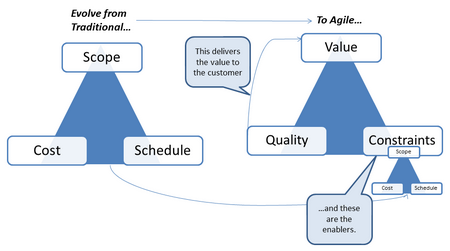
\includegraphics[width=0.7\linewidth]{figures/agile-triangle.png}
	\caption[Transitioning to Agile methodologies.]{Traditional to Agile project management evolution. Source: Agile Australia - Opening keynotes~\citep{web:AgileTriangle}}
	\label{fig:agile-pm}
\end{figure}

\section{Goals \& scope}
\label{Management:Scope}

One of the first things to do when beginning any project is delimiting its \textbf{scope}, this is, deciding \textit{what} will be done and \textit{how}, in terms of resources and methodology.

We already stated in \sref{Introduction::moa-ppsm} what the main \textit{goal} of this project is:

\begin{quote}
	\begin{description}
		\item[Main goal:] \hfill \\
		Implement privacy preserving filters for the Massive Online Analysis (MOA) stream mining framework.
	\end{description}
\end{quote}

\subsection{Requirements analysis}
\label{Management:Scope:Requirements}

For the sake of completeness and verbosity, a more detailed list of the project's \textit{requirements} is given in the next couple of sections, categorized into \textit{functional}\footnote{Functional requirements explain what has to be done by identifying the necessary task, action or activity that must be accomplished.} and \textit{non-functional}\footnote{Non-functional requirements are requirements that specify criteria that can be used to judge the operation of a system, rather than specific behaviors.} ones. Together, they comprise the formal scope of the project.

\subsubsection*{Functional requirements}

\begin{enumerate}[leftmargin=1.5cm, label=\textbf{R\arabic*}]
	\item
	Implement privacy preserving stream mining \textit{filters}\footnote{Within the MOA context, \textit{filters} are procedures applied to data prior to their analysis using machine learning algorithms.} for the MOA stream mining framework. The \textit{suggested} algorithms to be implemented correspond with the following requirements:
	\begin{enumerate}[label*=\textbf{-\arabic*}]
		\item Noise addition~\citep[p.~54]{Hundepool:StatisticalDisclosureControl}
		\item Multiplicative noise~\citep[p.~57]{Hundepool:StatisticalDisclosureControl}
		\item Microaggregation~\citep[p.~60]{Hundepool:StatisticalDisclosureControl}
		\item Rank swapping~\citep[p.~73]{Hundepool:StatisticalDisclosureControl}
		\item Differential privacy~\citep{Dwork:DifferentialPrivacy}
	\end{enumerate}
	
	\item
	Evaluate technological alternatives prior to the implementation of the privacy filters.
	
	\item
	Benchmark the performance of the filters in terms of \textit{disclosure risk} and \textit{information loss}.
\end{enumerate}

\subsubsection*{Non-functional requirements}

\begin{enumerate}[leftmargin=1.5cm, label=\textbf{NFR\arabic*}]
	\item
	\textit{Correctness:} privacy protection is at stake in this project, so algorithms must be implemented correctly, from the theoretical point of view, in order to not ease information disclosure when they are used.
	
	\item
	\textit{Efficiency:} given that no data mining process can scale well if its algorithms are slow, effort will be put in making them the most efficient we can.
	
	\item
	\textit{Test coverage:} measures and tests will be performed to assess the quality of the developed software, as well as its scalability and performance, which is paramount in this project’s context.
	
	\item
	\textit{Documentation:} MOA is an \textit{open source} data mining framework, which means that its community can assess how is it built and how to improve it. One of the benefits of the open source development model is that software can be safer, more robust and efficient, by receiving contributions from different developers. If people are to continue improving the work done, it has to be well documented.
\end{enumerate}

\subsection{Scope deviations}
\label{Management:Scope:Deviations}

There have been no major changes in the scope of the project along its development. Both the functional and non-functional requirements sets remain the same as the ones defined in the final report of the Project Management course (and also listed above).

However, concerning its completion, we have to admit that not all requirements have been achieved. We provide now an enumeration of the functional requirements and their final status:

\begin{enumerate}[leftmargin=1.5cm, label=\textbf{R\arabic*}]
	\item
	\textsc{[Mostly completed]} Implement privacy preserving stream mining \textit{filters} for the MOA stream mining framework.
	\begin{enumerate}[label*=\textbf{-\arabic*}]
		\item \textsc{[Completed]} Noise addition~\citep[p.~54]{Hundepool:StatisticalDisclosureControl}
		\item \textsc{[Not completed]} Multiplicative noise~\citep[p.~57]{Hundepool:StatisticalDisclosureControl}
		\item \textsc{[Completed]} Microaggregation~\citep[p.~60]{Hundepool:StatisticalDisclosureControl}
		\item \textsc{[Completed]} Rank swapping~\citep[p.~73]{Hundepool:StatisticalDisclosureControl}
		\item \textsc{[Completed]} Differential privacy~\citep{Dwork:DifferentialPrivacy}
	\end{enumerate}
	
	\item
	\textsc{[Completed]} Evaluate technological alternatives prior to the implementation of the privacy filters.
	
	\item
	\textsc{[Completed]} Benchmark the performance of the filters in terms of \textit{disclosure risk} and \textit{information loss}.
\end{enumerate}

Even though the \textbf{R1-2} requirement could not be finished, and further work would be possible, as will be discussed in the Conclusions section, the Agile approach for this project has enabled us to avoid a sense of failure at the end of its development.
\section{Methodology}
\label{Management:Methodology}

The methodology approach used in this project will be based on Agile principles. Some of the key concepts and practices related to Agile software development are:

\begin{itemize}
	\item \textbf{Iterative} development versus the classical \textit{waterfall} development model.
	\item Short to mid range development \textbf{sprints} (phases), in order to keep track of the project’s evolution and to be able to react to changes, unforeseen constraints or scope drifts.
	\item \textbf{Constant meetings} with the project’s stakeholders, in which the progress and deviations of the project are assessed.
	\item Usage of \textbf{burndown charts} - a graphical model of work left to do versus time - and other visual representations of the project's track
	\item Reduced documentation generation, to alleviate the potential loss of time that changes in the requirements would cause.
\end{itemize}

Among many other approaches and Agile methodological frameworks, \textit{Scrum} is one of the most well-known due its flexibility, its proved resilience against requirements rapid changes and easy adoption by software development teams.

\subsection{Scrum}

\textbf{Scrum} is an iterative and incremental agile software development methodology for managing product development. It challenges assumptions of the \textit{traditional, sequential approach} to product development, and enables teams to self-organize by encouraging physical location or close online collaboration of all team members, as well as daily face-to-face communication among all team members and disciplines in the project~\citep{web:Wiki:Scrum}.

\begin{figure}
	\centering
	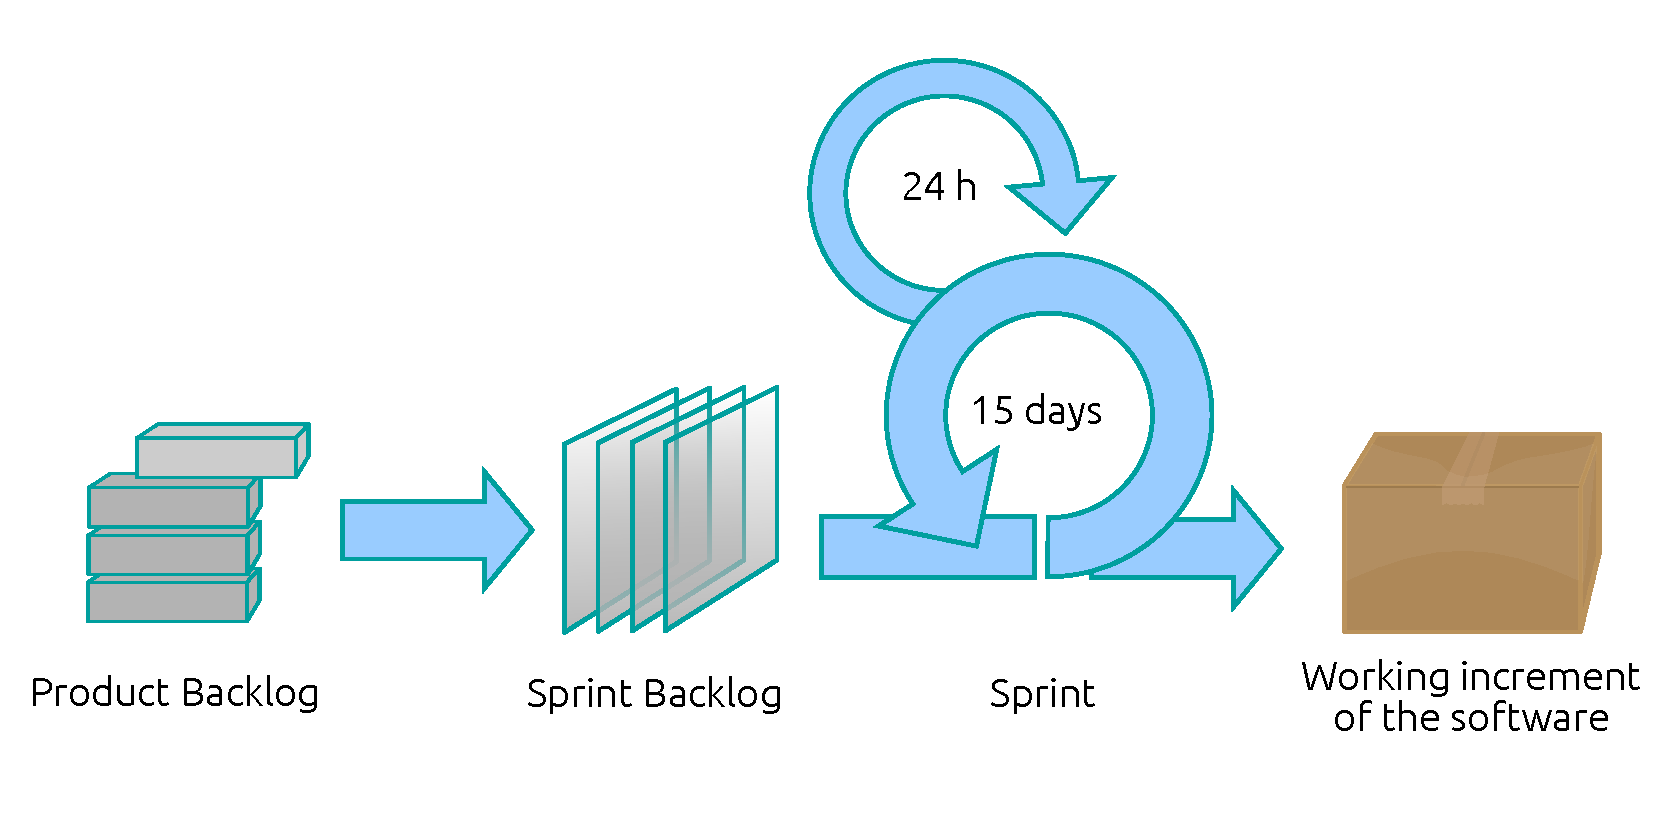
\includegraphics[width=0.8\linewidth]{figures/scrum.pdf}
	\caption{\textit{Scrum} methodology process overview. Adapted from Wikimedia~\citep{web:Wiki:ScrumProcess}}
	\label{fig:scrum}
\end{figure}

This methodology is based on the adoption of certain roles, as well as some \textit{artifacts} and predefined processes, all of which can be adapted as necessary by the team to suit their specific needs and resources. However, a central concept forms the basis for the rest of the framework: the \textbf{sprint}. A sprint or iteration is the basic unit of development in Scrum. The sprint is a timeboxed effort, this is, it is restricted to a specific duration, which is fixed in advance for each sprint and is normally between one week and one month, with two weeks being the most common.

\subsubsection*{Roles}

The follwing are the relevant roles that emerge in a Scrum developed project:

\begin{itemize}
	\item
	\textbf{Product owner:} the product owner represents the stakeholders and is the voice of the customer. He or she is accountable for ensuring that the team delivers value to the business. The product owner writes \textit{user stories} (tasks) and adds them to the \textit{product backlog}, prioritizing them.
	
	\item
	\textbf{Scrum master:} Scrum is facilitated by a scrum master, who is accountable for removing impediments to the ability of the team to deliver the product goals and deliverables. The scrum master is not a traditional team lead or project manager, but acts as a buffer between the team and any distracting influences. The scrum master ensures that the scrum process is used as intended.
	
	\item
	\textbf{Development team:} the development team is responsible for delivering potentially shippable increments of product at the end of each \textit{sprint}. A team is made up of 3–9 individuals with cross-functional skills who do the actual work: analyse, design, develop, test, document, etc. Finally, it is important to emphasize that the development team in Scrum is self-organizing.
\end{itemize}

\subsubsection*{Events}

A series of \textit{events} take place during the Scrum process, configuring the actual workflow of the team. We will provide an overview of some of them:

\begin{itemize}
	\item
	\textbf{Sprint planning:} at the beginning of a sprint, the team holds a sprint planning event, in which the work to be done is selected from the product backlog and transferred to the sprint backlog.
	
	\item
	\textbf{Daily Scrum:} a stand-up, timeboxed and short meeting takes place every day during each sprint. In these meetings, every member of the team explains the work carried out the previous day, discusses any impediment or blocking situation he or she has encountered and decides which tasks will do in the following day.
	
	\item
	\textbf{Retrospective:} at the end of each sprint, a review of the work that has been completed is made, and the team reflects on the past sprint to identify and agree on any process improvement, which requires actions to be taken in the upcoming sprint.
\end{itemize}

\subsubsection*{Artifacts}

Even though we have given an overview of some of them, the following artifacts are the remaining pieces that shape up the Scrum process and methodology:

\begin{itemize}
	\item
	\textbf{Product backlog:} the product backlog is an ordered list of requirements that is maintained for a product. It consists of features, bug fixes, non-functional requirements, etc., i.e., whatever needs to be done in order to successfully deliver a viable product. The items in this backlog are ordered by the product owner based on considerations like risk, business value, dependencies or date needed, for example.
	
	\item
	\textbf{Sprint backlog:} The sprint backlog is the list of work the development team must address during the next sprint. The list is derived by selecting product backlog items from the top of the product backlog until the development team feels it has enough work to fill the sprint. The development team should keep in mind its past performance assessing its capacity for the new sprint, and use this as a guide line of how much \textit{effort} they can complete.
\end{itemize}

\subsection{Agile in this project}

The methodology chosen for this project will be based upon Scrum, but major modifications will have to be made, for a number of reasons. Firstly, there is no such \textit{development team}: a single developer will take care of the implementation of the project. Moreover, there is no possibility of having a Scrum master either. The project director will take a role between a technical coordinator and a product owner, although no real concept of \textit{product} exists in the project, either way.

\subsubsection{Practices}

The adopted Agile practices for this project include:

\begin{itemize}
	\item The usage of Trello\footnote{Its description, along with other resources and tools used, can be found on~\sref{Management:Budget:Resources}} as a task tracking tool, to prioritize them similarly to the Scrum backlogs.
	\item \textbf{Sprint}-based development cycles with a sprint duration of one week.
	\item Constant (re)-evaluation of constraints and requirements, to forsee changes and take preventive action (similar to retrospectives, but less formal and certainly shorter).
\end{itemize}

\subsubsection{Scope}

Adopting Agile methodologies involves several decisions on how to manage the project and its requirements. In this particular project, if we are to examine the classical constraints (of which we talked about at the beginning of this chapter), we must be aware that the \textit{schedule is fixed} (perhaps not the planning, but the final milestone) and this forces us to let the \textbf{scope opened}. This means that we will implement as much features as we can, assessing their quality, but no feature list will drive the success or failure of the project. Because we will be working on the basis of such an \textit{open scope}, deviations in this field are likely to happen. These, however, will not result in a project failure in any case, because an agreement has been reached to work this way.
\section{Schedule}
\label{Management:Schedule}

The following subsections provide some details about the initial project planning (\sref{Management:Schedule:Initial}), as well as the changes it has suffered over time (\sref{Management:Schedule:Final}). There have been \textit{significant} deviations concerning the original project schedule. Not only the global duration has been lengthened, but more phases have been layed out, as was needed. As a positive contrast, early detection of such alterations has been sometimes possible.

\subsection{Initial schedule}
\label{Management:Schedule:Initial}

In this section, we cover the original analysis that was reported during the Project Management module\footnote{The Project Management module is a compulsory course that all students have to undertake when beginning their Bachelor's Degree Final Project, concerning project management concepts and techniques, as well as documentation.}, at the beginning of this project's development.

\subsubsection{Overall duration}

Taking a general look at the project’s schedule, we can estimate it to have a total duration of about 5 months. Even though it was registered on July, 2014, the project did not begin until September, because August is the only month I can have holidays, due to job restrictions. Considering the next possible project’s lecture shifts, we believe that the one taking place in December is too close in time. Thus, the project will endure until January the 26th, 2015. This should give us time enough to develop the project and document it without too much pressure, which is key to fulfill one of the main established goals: high quality results.

\subsubsection{Schedule slack}

The project schedule we present herein does not fill up the total amount of time available - more than two weeks are left blank, with no assigned tasks. This is intended because of the following reasons:

\begin{itemize}
	\item The amount of time needed to develop the proposed algorithms is uncertain. It is hard to estimate the time it may take, because I have no previous knowledge on the area. Therefore, we opted for, in one hand, an \textit{open scope} approach, and, on the other, leaving a considerable time gap between the last planned task and the project’s final milestone: its defense. Being conservative, if the development of any proposed method is delayed, we still have some leeway to introduce schedule changes, without risking the project’s success.
	
	\item We have estimated the project’s report confection and the defense presentation rehearsals to be 35 and 7 days, respectively, but depending on how much development is finally carried out, it might not be time enough to write down the report. Extra time for doing it can be then borrowed from the schedule slack time.
	
\end{itemize}

\subsubsection{Schedule monitoring \& changes}

For the development phase of the project, the most suitable way to monitor the schedule we have found is applying an Agile approach to the process. We will work in one week long sprints, meeting every week to assess the quality of the solutions, the proper progress of the project and to plan what will be done during the following sprint.

Sprint planning meetings are where the main goals of the project will be sliced in small tasks, which can be tracked and implemented better, because they are not so complex. Thanks to this constant fine-grained planning process, schedule or scope deviations are detected earlier and can be managed efficiently, reacting before they affect deeper the overall success of the project. Given that no fixed features list is assigned to each sprint of the development phase, if the completion of either of those features is delayed, it can be made to span for some more time.

Within each of the development sprints, burndown charts\footnote{A burn down chart is a graphical representation of work left to do versus time. The outstanding work (or backlog) is often on the vertical axis, with time along the horizontal. That is, it is a run chart of outstanding work. It is useful for predicting when all of the work will be completed. It is often used in agile software development methodologies such as Scrum.} will be used to monitor the progress of the sprint. These charts are helpful in identifying patterns of work (sprint-end rushes, for example) and can help developers maintain a constant rate of finished features.

Besides burndown charts and sprint planning meetings, the use of velocity charts will also be helpful to increase the predictability of the following sprint plannings. The more predictable they are, the less deviations will occur and the schedule will be more likely to be fulfilled.

\subsubsection{Project phases}

The project is divided in 4 main phases, besides of the undertaking of the Project's Management module. Each phase has an estimated duration and a risk evaluation in terms of schedule deviation. The amount of hours is an approximated calculation from the number of days in each phase: 4 hours a day are estimated to be spent, because I am currently working part-time and also taking some subjects. A more detailed task granularity can be seen in the Gantt chart (on \fref{fig:gantt-1} and~\fref{fig:gantt-2}). Task dependencies are shown in the chart too. Those phases, chronologically ordered are:

\begin{enumerate}[leftmargin=1.5cm, label=\textbf{{[}Phase \arabic*{]}}]
	\item \textbf{Contextualization}: it is intended to perform a deeper bibliographic research and a study of the main subjects concerning the project, at the theory level - no practical skills or technological research will be done.
	\begin{itemize}
		\item \textbf{Duration estimation:} 11 days (44 hours).
		\item \textbf{Risk:} this phase has a medium to high risk of being delayed, due to lack of effective time (a wrong estimation), and also because more insight than planned might be needed, consuming more time.
	\end{itemize}
	
	\item \textbf{Environment setup}: during this phase, all necessary tools and material resources will be gathered and configured. The concrete developing workflow will be decided, too.
		\begin{itemize}
			\item \textbf{Duration estimation:} 8 days (32 hours).
			\item \textbf{Risk:} this phase has a low risk of being delayed, because the technology that is to be used is, a priori, well known to us.
		\end{itemize}
		
	\item \textbf{Development}: all of this project coding will be performed during this phase. As said before, a sprint methodology will be used during this phase, being one week each.
		\begin{itemize}
			\item \textbf{Duration estimation:} with an initial planning of 7 sprints, 49 days will be used (196 hours).
			\item \textbf{Risk:} there is a medium risk of this phase to be delayed. Even with the use of Agile methodologies, if a fundamental feature was needed and there was no more time left, another sprint (or at most a couple of them) could be introduced, to finish the remaining tasks.
		\end{itemize}
		
	\item \textbf{Documentation}: the project’s report will be written after the development phase, along with any deployment documentation that was required and the final presentation, which will also be rehearsed then.
		\begin{itemize}
			\item \textbf{Duration estimation:} 42 days (168 hours).
			\item \textbf{Risk:} this phase has a medium risk of being delayed too. Reviews of the report will be made and writing in English might take up more time than expected.
		\end{itemize}
	
\end{enumerate}

\subsubsection{Detailed schedule: Gantt chart}

A detailed Gantt chart of the schedule can be seen in~\fref{fig:gantt-1} and~\fref{fig:gantt-2}. The chart was generated with the \textit{Project management} free software package, available online on the Ubuntu 12.04 Software Center. Please note that there is no way the chart could fit in a single page (not even if it was landscape).

\begin{figure}[hbtp]
	\makebox[\textwidth]{
		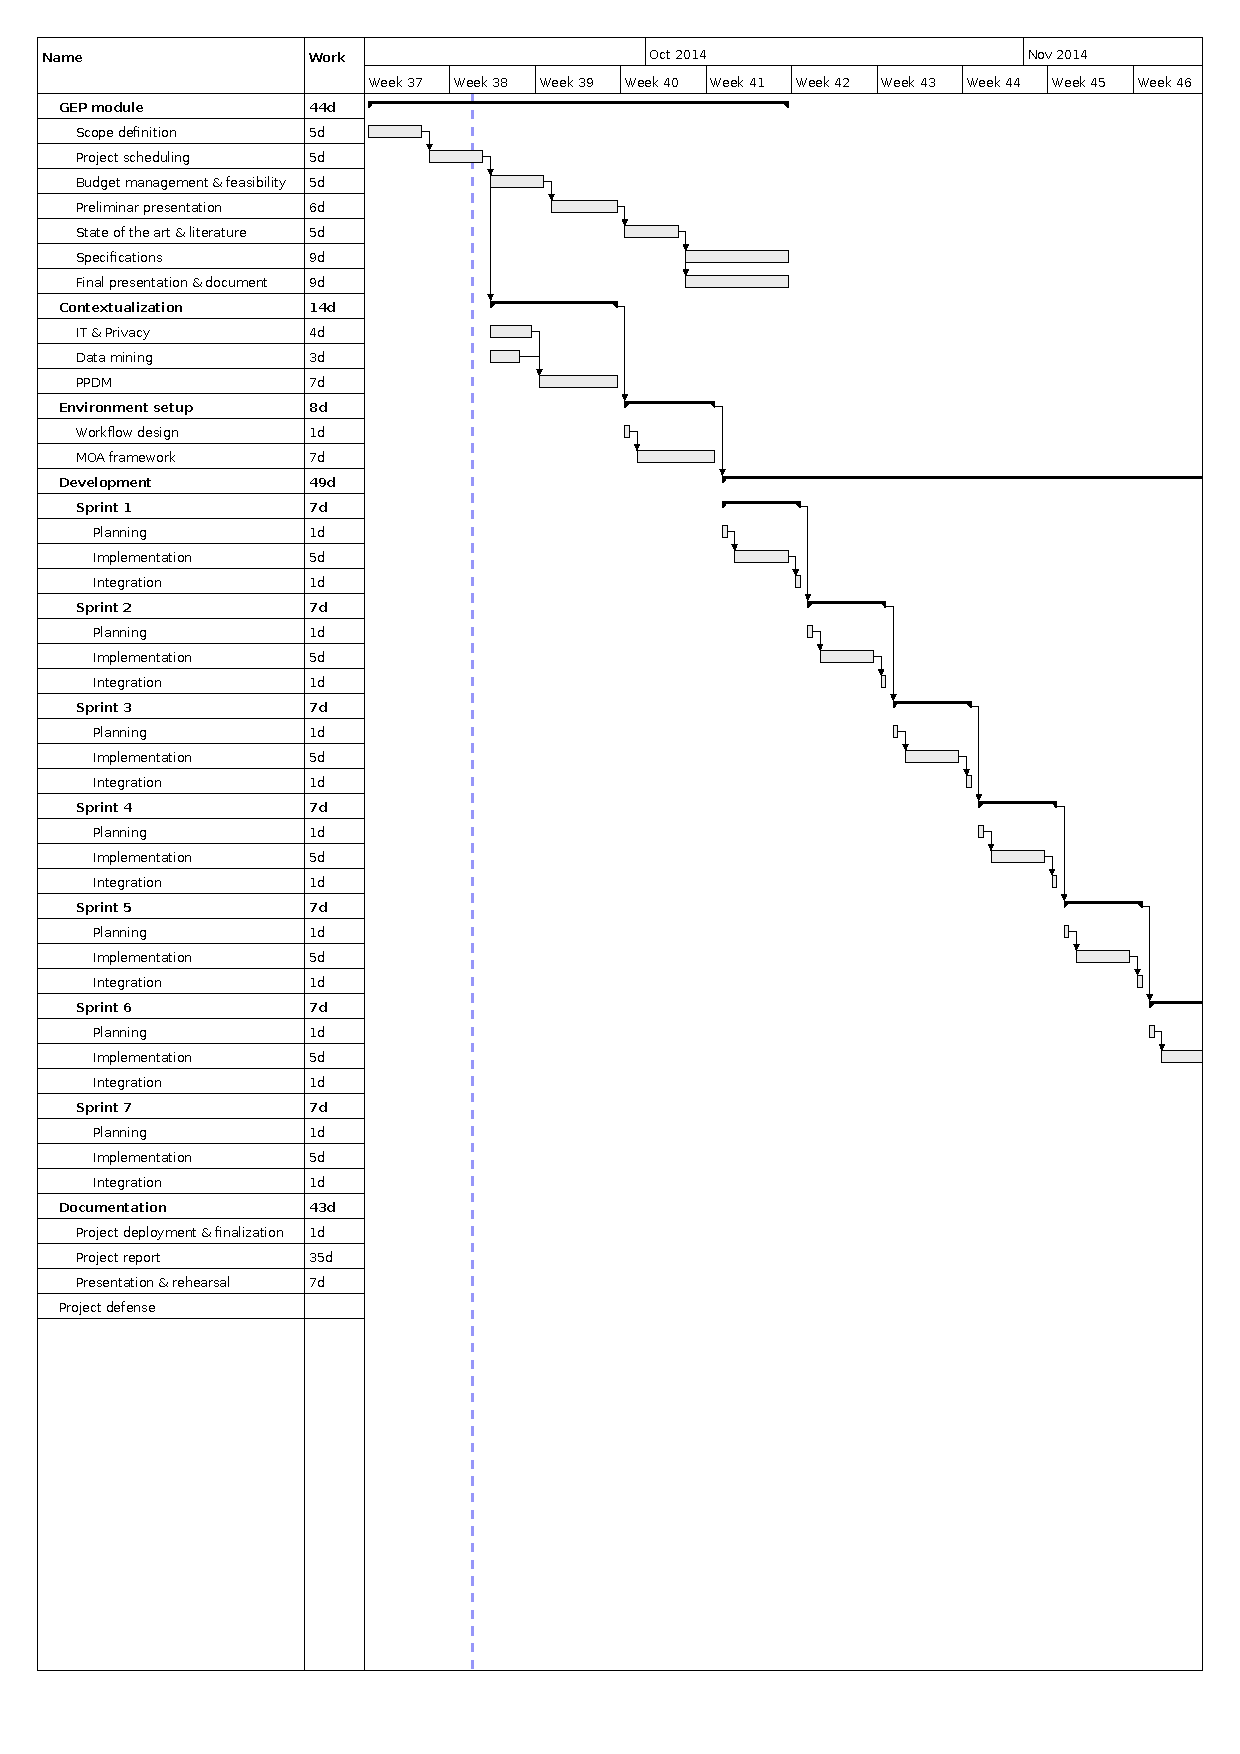
\includegraphics[trim={0 7.3cm 0 0},clip,page=1,width=1.2\linewidth]{figures/gantt-chart.pdf}
	}
	\caption{Initial project schedule Gantt chart (part 1).}
	\label{fig:gantt-1}
\end{figure}

\begin{figure}[hbtp]
	\makebox[\textwidth]{
		\includegraphics[trim={0 7.3cm 0 0},clip,page=2,width=1.2\linewidth]{figures/gantt-chart.pdf}
	}
	\caption{Initial project schedule Gantt chart (part 2).}
	\label{fig:gantt-2}
\end{figure}

\clearpage

\subsection{Schedule deviation}
\label{Management:Schedule:Final}

We will cover now the changes that have occurred in the schedule of the project and analyze its causes.

\subsubsection{Overall duration}

The original total duration has been extended from 5 months to 8 months, approximately. Thus, the final report and its defence is now scheduled to be in April, which is the next available lecture shift in the Faculty. We believe that this extended duration will allow us to fulfill all requirements defined in the scope of the project.

\subsubsection{Deviation analysis}

There are several possible reasons behind this schedule deviation:

\begin{itemize}
	\item The Project Management module lasted longer than expected, forcing the development phase of the project to begin later.
	\item During the definition of the project initial schedule, we expected to begin developing it while the Project Management module endured, which was, definitely, a planning error. Such tasks concurrency was not possible at that time.
	\item At the beginning of the development phase, we explored different technological alternatives, before deciding which approach was mostly suited to our needs, but this exploration delayed the actual development process for a couple of weeks.
	\item As was already stated in the Project Management report, some of the requested features have posed to be more complicated than was expected, consuming some more time than that assigned to them.
	\item For personal reasons, no work could be carried out during the Christmas vacations, which lasted two more weeks, furtherly delaying the project's development.
\end{itemize}

\subsubsection{Current detailed schedule}

Considering the previous analysis, a new Gantt chart has been built, with the new project's schedule, which is detailed in~\fref{fig:new-gantt-1} and~\fref{fig:new-gantt-2}.

\begin{figure}[hbtp]
	\makebox[\textwidth]{
		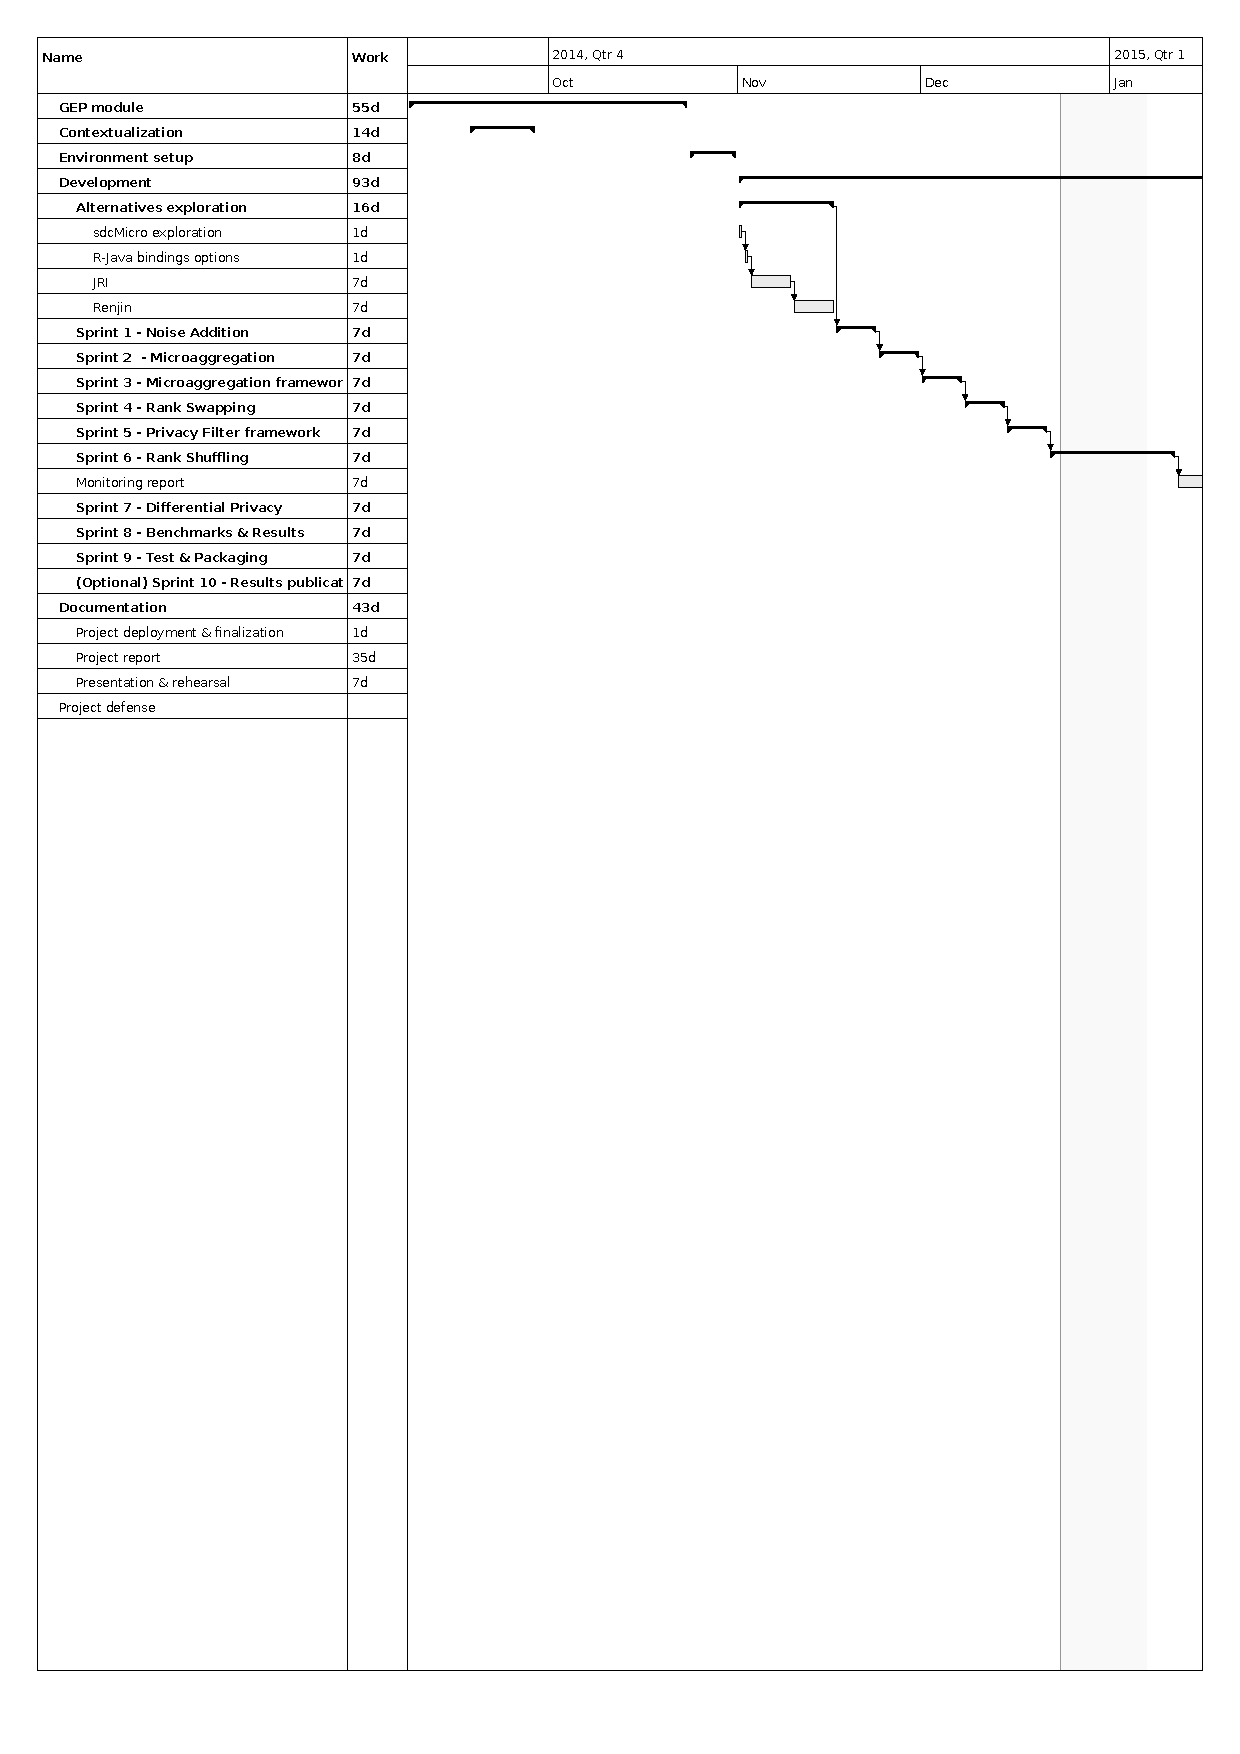
\includegraphics[angle=90,trim={0 17.5cm 0 0},clip,page=1]{figures/new-gantt-chart.pdf}
	}
	\caption{Final project schedule Gantt chart (part 1).}
	\label{fig:new-gantt-1}
\end{figure}

\begin{figure}[hbtp]
	\makebox[\textwidth]{
		\includegraphics[angle=90,trim={0 17.5cm 0 0},clip,page=2]{figures/new-gantt-chart.pdf}
	}
	\caption{Final project schedule Gantt chart (part 2).}
	\label{fig:new-gantt-2}
\end{figure}

\clearpage
\section{Budget}
\label{Management:Budget}

The initial budget and resources analysis, performed during the Project Management module, corresponds with~\sref{Management:Budget:Resources},~\sref{Management:Budget:Estimation} and~\sref{Management:Budget:Control}. Due to schedule deviations during the project, a final budget estimation is given in~\sref{Management:Budget:Final}.

The project’s budget is entirely based on an estimation of human, hardware and software resources costs. No real income is perceived, besides the salary of the project’s supervisor, who is a tenure-track lecturer at the Barcelona School of Informatics, and an associate researcher at the Barcelona Supercomputing Center. No third parties are involved in the project - no companies or organizations are providing any funds. Moreover, even though the work is to be integrated into the MOA framework, it is indeed an open-source project, to which we will be contributing, meaning contributions are expected from any kind of source, be it funded or not.

All other associated costs are \textit{externalized}, either by people involved in the project or by the university, where the development of the project will be held.

\subsection{Resources \& budget estimation}
\label{Management:Budget:Resources}

Resources consumed in this project only fall in one of the following categories: \textit{human resources}, \textit{hardware}, \textit{software} and \textit{other expenses}. For a detailed description of what will be needed in the project, please see the following subsections. It is important to keep in mind that \textit{all} resources will be consumed equally througout the entire project duration.

\subsubsection{Human resources}

Human resources are summarized in~\tref{table:human-resources}.

All expenses included here are related to people’s salaries. Only one developer will be working on this project, but a number of hours involving supervision tasks is also imputed to the project’s supervisor, so its corresponding cost is added too. Taxes are included in all of the following items. The price is also an estimation: on the developer’s side, it is based on a salaries comparison webpage (\textit{Glassdoor}~\citep{web:Glassdoor})\footnote{As of date 12th October, 2014, the average salary for a software engineer in Barcelona is 32000€ per year (including taxes). Considering 12 monthly instalments and an average of 160 hours per month, this yields a total of 16.66€ per hour.}; on the supervisor side, the price is based on his own estimation.

\begin{itemize}
	\item \textbf{Developer:} an average of 20 hours a week are estimated, spanning for about 21 weeks, summing up a total of 420 hours.
	\item \textbf{Supervisor:}
	\begin{itemize}
		\item \textbf{Project’s take off:} 8 hours, between meetings and initial planning.
		\item \textbf{Sprints:} 8 hours each sprint, taking into account both face to face meetings and other supervising tasks. There are 7 sprints scheduled so far, making a total of 56 hours.
		\item \textbf{Documentation:} during the project’s final stage, an estimation of 20 hours is taken from the corresponding supervision of the project’s report.
	\end{itemize}
\end{itemize}

\begin{table}[h]
	\centering
	\begin{tabular}{lllr}
		\hline
		\textbf{Role} & \textbf{Price (per hour)} & \textbf{Working  hours} & \multicolumn{1}{l}{\textbf{Total}} \\ \hline
		Supervisor & \multicolumn{1}{r}{35€} & \multicolumn{1}{r}{84} & 2940€ \\
		Developer & \multicolumn{1}{r}{16.66€} & \multicolumn{1}{r}{420} & 6997.2€ \\ \hline
		&  & \multicolumn{1}{r}{\textbf{Total}} & \textbf{9937.2€}
	\end{tabular}
	\caption{Human resources associated costs. All taxes are included in the Price per hour column.}
	\label{table:human-resources}
\end{table}

\subsubsection{Hardware resources}

Hardware resources are summarized in~\tref{table:hardware-resources}.

All hardware needed resources are shown in the corresponding table. Their cost is calculated by estimating its amortization, spanned over 5 years (it is a personal laptop). To calculate its amortized cost per hour, we will take into account that this equipment is used throughout the course too, and estimating that 2500 hours of work are carried each year.

\begin{table}[h]
	\centering
	\begin{tabular}{l r r r r r}
		\hline
		\textbf{Product} & \multicolumn{1}{l}{\textbf{Price}} & \multicolumn{1}{l}{\textbf{Units}} & \multicolumn{1}{p{3cm}}{\textbf{Amortized price per hour}} & \multicolumn{1}{l}{\textbf{Work time (hours)}} & \multicolumn{1}{l}{\textbf{Total}} \\ \hline
		Asus k53sv & 650€ & 1 & 0.052€ & 420 & 21.84€ \\ \hline
		&  &  &  & \textbf{Total} & \textbf{21.84€}
	\end{tabular}
	\caption{Hardware amortization costs. All taxes included.}
	\label{table:hardware-resources}
\end{table}

\subsubsection{Software resources}

All software needed to undertake this project is free and, most of it, is open sourced. Despite this, we will include a list of it here, to show what will be used at a finer grain.

\begin{itemize}
	\item \textbf{Ubuntu 12.04}: operating system. Available at: \url{http://www.ubuntu.com/download}.
	\item \textbf{Trello}: online task management tool. Available at: \url{https://trello.com/}.
	\item \textbf{Google Drive}: online, collaborative office software suit, used to create burndown charts (spreadsheets). Available at: \url{https://drive.google.com}.
	\item \textbf{Java SDK}: Java language Software Development Kit. Available at: \url{http://openjdk.java.net}.
	\item \textbf{Eclipse IDE}: integrated development environment package. Available at: \url{https://www.eclipse.org/home/index.php}.
	\item \textbf{Git}: source version control system. Available at: \url{http://git-scm.com/}. Remote code repositories will be hosted at GitHub (\url{https://github.com}) for free.
	\item \textbf{MOA}: Massive Online Analysis, a stream mining framework. Available at: \url{http://moa.cms.waikato.ac.nz}.
	\item \textbf{\LaTeX}: document preparation system. Available at: \url{http://www.latex-project.org}.
\end{itemize}

\subsubsection{Other expenses}

All expenses not covered in the previous sections are detailed in~\tref{table:other-resources}.

\textbf{Please note} that the cost of each item of this section is an estimation. Moreover, even though they are displayed, since no budget is really available, they will be \textit{absorbed} by the university, where most of the work will be carried out.

\begin{table}[h]
	\centering
	\begin{tabular}{lrrr}
		\hline
		\textbf{Product} & \multicolumn{1}{l}{\textbf{Price per month}} & \multicolumn{1}{l}{\textbf{Months}} & \multicolumn{1}{l}{\textbf{Total}} \\ \hline
		Energy & 35€ & 4 & 140€ \\
		Water & 25€ & 4 & 100€ \\
		Heat \& air & 30€ & 4 & 120€ \\
		Internet connection & 40€ & 4 & 160€ \\ \hline
		& \multicolumn{1}{l}{} & \textbf{Total} & \textbf{520€}
	\end{tabular}
	\caption{Uncategorized resources estimated costs. All taxes are included.}
	\label{table:other-resources}
\end{table}

\subsection{Total budget estimation}
\label{Management:Budget:Estimation}

The sum of the subtotals of the previous sections is shown in~\tref{table:total-resources}. Please note that, since taxes are already included in each item appropriately, there is no need to add them here.

\begin{table}[h]
	\centering
	\begin{tabular}{lr}
		\hline
		\textbf{Concept} & \multicolumn{1}{l}{\textbf{Total}} \\ \hline
		Human resources & 9937.2€ \\
		Hardware & 21.84€ \\
		Software & 0€ \\
		Other expenses & 520€ \\ \hline
		\multicolumn{1}{r}{\textbf{Total}} & \multicolumn{1}{l}{\textbf{10479.04€}}
	\end{tabular}
	\caption{Total budget: summation of budget estimations.}
	\label{table:total-resources}
\end{table}

All costs are just estimations and are not covered in any way, with the exception of the supervisor’s salary. This means that, in fact, there is no possible way this project is feasible. However, given that the developer has no salary at all and that all other extra costs are assumed by the university or the developer, the project can be developed normally.

\subsection{Budget control mechanisms}
\label{Management:Budget:Control}

Any budget deviations related to material equipment or software purchases will be monitored in the sprint planning meetings at the beginning of each of those phases during the project. These possible extra costs will be assumed by the developer, since no other source of funds is available.

Another source of budget deviations can be found on the project’s duration. If the schedule is not fulfilled and the project is delayed, extra cost in terms of human resources, hardware amortizations and other expenses would have to be added. They still would be treated as they are in the present analysis, meaning no significant change would occur.

\subsection{Final budget estimation}
\label{Management:Budget:Final}

Due to the deviation in the project's schedule, that was already analyzed in~\sref{Management:Schedule:Final}, an increment in the human resources, external expenses and hardware amortization budget contributions has arised. It is important to note that, given that no proprietary software package has been used, no additional costs might be derived from the lenghtening of the project duration. We will now cover this budget deviation and provide a final estimation of the project cost, which is summarized in~\tref{table:final-total-resources}.

\subsubsection*{Human resources: deviation}

Following the analysis from~\ref{Management:Budget:Resources}, we just have to add the corresponding increment of working hours for both the developer and supervisor.

\begin{itemize}
	\item \textbf{Developer:} an average of 20 hours a week are estimated, spanning for about 32 weeks, summing up a total of 640 hours. However, given that no work was carried during Christmas holidays, the total number of hours should be lowered to, at most, \textbf{600 hours}.
	\item \textbf{Supervisor:}
	\begin{itemize}
		\item \textbf{Project’s take off:} 8 hours, between meetings and initial planning.
		\item \textbf{Sprints:} 8 hours each sprint, taking into account both face to face meetings and other supervising tasks. With 10 sprints of final work, this yields a total of \textbf{80 hours}.
		\item \textbf{Documentation:} during the project’s final stage, an estimation of \textbf{20 hours} is taken from the corresponding supervision of the project’s report.
	\end{itemize}
\end{itemize}

Considering the previous estimation and keeping the same prices per hour of the initial estimation, the following total human resources cost is calculated (see~\tref{table:human-resources-final}).

\begin{table}[h]
	\centering
	\begin{tabular}{lllr}
		\hline
		\textbf{Role} & \textbf{Price (per hour)} & \textbf{Working  hours} & \multicolumn{1}{l}{\textbf{Total}} \\ \hline
		Supervisor & \multicolumn{1}{r}{35€} & \multicolumn{1}{r}{108} & 3780€ \\
		Developer & \multicolumn{1}{r}{16.66€} & \multicolumn{1}{r}{600} & 9996€ \\ \hline
		&  & \multicolumn{1}{r}{\textbf{Total}} & \textbf{13776€}
	\end{tabular}
	\caption{Human resources associated costs (final estimation).}
	\label{table:human-resources-final}
\end{table}

\subsubsection*{Hardware resources: deviation}

The only change in the hardware related costs is the number of working hours devoted to the project, which have a direct impact on the amortization of the equipment.

\begin{table}[h]
	\centering
	\begin{tabular}{l r r r r r}
		\hline
		\textbf{Product} & \multicolumn{1}{l}{\textbf{Price}} & \multicolumn{1}{l}{\textbf{Units}} & \multicolumn{1}{p{3cm}}{\textbf{Amortized price per hour}} & \multicolumn{1}{l}{\textbf{Work time (hours)}} & \multicolumn{1}{l}{\textbf{Total}} \\ \hline
		Asus k53sv & 650€ & 1 & 0.052€ & 600 & 31.2€ \\ \hline
		&  &  &  & \textbf{Total} & \textbf{31.2€}
	\end{tabular}
	\caption{Hardware amortization costs (final estimation).}
	\label{table:hardware-resources-final}
\end{table}

\subsubsection*{Other expenses: deviation}

Given that the amount of months dedicated to the project's development has increased, the estimated cost for the expenses related to the developer's accomodation has to reflect the changes as well.

\begin{table}[h]
	\centering
	\begin{tabular}{lrrr}
		\hline
		\textbf{Product} & \multicolumn{1}{l}{\textbf{Price per month}} & \multicolumn{1}{l}{\textbf{Months}} & \multicolumn{1}{l}{\textbf{Total}} \\ \hline
		Energy & 35€ & 7 & 245€ \\
		Water & 25€ & 7 & 175€ \\
		Heat \& air & 30€ & 7 & 210€ \\
		Internet connection & 40€ & 7 & 280€ \\ \hline
		& \multicolumn{1}{l}{} & \textbf{Total} & \textbf{910€}
	\end{tabular}
	\caption{Uncategorized resources estimated costs. All taxes are included.}
	\label{table:other-resources-final}
\end{table}

\clearpage

\subsubsection*{Final estimation}

The following is the final estimation of the project's budget, taking into account all deviations from the particular budget contributions.

\begin{table}[h]
	\centering
	\begin{tabular}{lr}
		\hline
		\textbf{Concept} & \multicolumn{1}{l}{\textbf{Total}} \\ \hline
		Human resources & 13776€ \\
		Hardware & 31.2€ \\
		Software & 0€ \\
		Other expenses & 910€ \\ \hline
		\multicolumn{1}{r}{\textbf{Total}} & \multicolumn{1}{l}{\textbf{14717.2€}}
	\end{tabular}
	\caption{Total budget final estimation.}
	\label{table:final-total-resources}
\end{table}